\documentclass{standalone}
\usepackage{tikz}
  \usetikzlibrary{positioning}
  \usetikzlibrary{arrows.meta}
  \usetikzlibrary{arrows, shapes, trees, positioning, decorations.markings, patterns}
  \usetikzlibrary{backgrounds}
  \usetikzlibrary[topaths]
  \usetikzlibrary{calc}
  \usetikzlibrary{backgrounds,fit,decorations.pathreplacing}
  \usetikzlibrary{shapes.multipart}
\usepackage{fontspec}
  \setmainfont[Ligatures=TeX]{Nimbus Roman No9 L}

\newcount\mycount

\usepackage{graphicx}
\graphicspath{{}{./assets/}}

\begin{document}
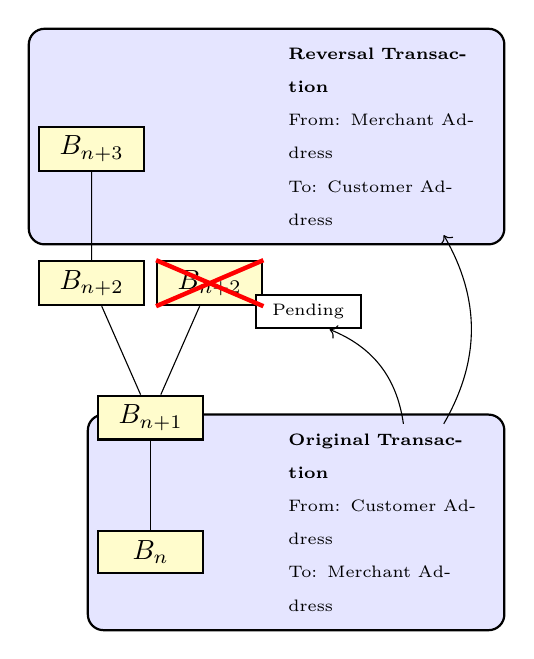
\begin{tikzpicture}[
    level distance=2cm,
    every label/.style={blue},
% Event style
    event/.style={rectangle,thick,draw,grow=up,fill=yellow!20,text width=1.1cm,
		text centered,font=\sffamily,anchor=north},
    event2/.style={rectangle,thick,draw,grow=up,fill=white!20,text width=0.6cm,
		text centered,font=\sffamily,anchor=north,font={\fontsize{6pt}{12}\selectfont},
		level distance=1cm},
    font={\fontsize{9pt}{12}\selectfont}
    ]

  \tikzstyle{surround} = [fill=blue!10,thick,draw=black,rounded corners=2mm]

  % \draw [thick, gray, dotted, shift={(0.25,0.25)}] (-2, -1) grid [xstep=0,ystep=1.25] (7, 5.5);
  \node (s0) [event] {$B_n$} [grow=up]
    child {
      node (s1) [event] {$B_{n+1}$}
      child {
	node (s12) [event] {$B_{n+2}$}
      }
      child {
	node (s22) [event] {$B_{n+2}$}
	child {
	  node (s3) [event] {$B_{n+3}$}
	}
      }
    };

  % \draw[->] (s0) edge[bend right, below] node{Original Transaction} (b1);
  % \draw[->] (b8) edge[bend right, above] node{Reversal Transaction} (s41);

  \node (tx2) at (3, 5) [text width=2.5cm,font={\fontsize{6pt}{12}\selectfont}] {\textbf{Reversal Transaction} \\ From: Merchant Address \\ To: Customer Address};
  \node (tx1) at (3, 0.1) [text width=2.5cm,font={\fontsize{6pt}{12}\selectfont}] {\textbf{Original Transaction} \\ From: Customer Address \\ To: Merchant Address};
  \node (p) [event,fill=white,font={\fontsize{6pt}{12}\selectfont}] at (2, 3) {Pending};
  \draw[->] (tx1) edge[bend right, below] node{} (p);
  \draw[->] (tx1) edge[bend right, below] node{} (tx2);

\draw[red,ultra thick] (s12.south west) -- ($(s12.north east)-(0pt,0pt)$);
\draw[red,ultra thick] ($(s12.north west)-(0pt,0pt)$) -- (s12.south east);

  % \node (c2) at (5, 2.1) {Voting $V_{n+2}$};
  % \node (c4) at (5, 4.5) {Voting $V_{n+4}$};
% \node (v1) [rectangle,fill=black!40,minimum width=3cm] at (0, 2.2) {44444};

\begin{pgfonlayer}{background} 
  \node[surround] (background) [fit = (s3) (tx2)] {};
\end{pgfonlayer}
\begin{pgfonlayer}{background} 
  \node[surround] (background) [fit = (s0) (tx1)] {};
\end{pgfonlayer}

\end{tikzpicture}
\end{document}
